\chapter{Descrição das atividades desenvolvidas no estágio}
% ---
Neste capítulo são descritas, de modo detalhado, todas as atividades desenvolvidas pelo aluno Dennis Teles dos Santos durante o período de estágio pelo programa de Iniciação Científica ligado ao projeto CITAR no âmbito da meta 2, realizado no laboratório NSEE do Instituto Mauá de Tecnologia.

% ---
\section{Introdução}
Durante o período de estágio, o aluno participou do programa de Iniciação Científica financiado pelo CNPq, sob orientação do professor Vanderlei Cunha Parro e da coorientação do Engenheiro Rafael Corsi Ferrão formado pela Mauá no ano de 2011.

Para a realização e conclusão do projeto o aluno desempenhou as seguintes atividades: Construção de um hardware, firmware e software.
% ---

% ---
\section{Objetivo}

O projeto está no âmbito da meta 2 do projeto CITAR (ver figura \ref{Meta2}) e tem como objetivo desenvolver um hardware de uso de bancada capaz de ler e escrever em conversores A/D e D/A e em saídas e entradas digitais. O dispositivo será conectado em um nó SpaceWire (protocolo de comunicação aeroespacial amplamente utilizado). A arquitetura proposta do projeto pode ser visualizada na figura \ref{ArchSpW}.

\afterpage{	% \afterpage
\begin{figure}[!htb]
	\centering
	\caption{Projeto CITAR - Meta 2.}
	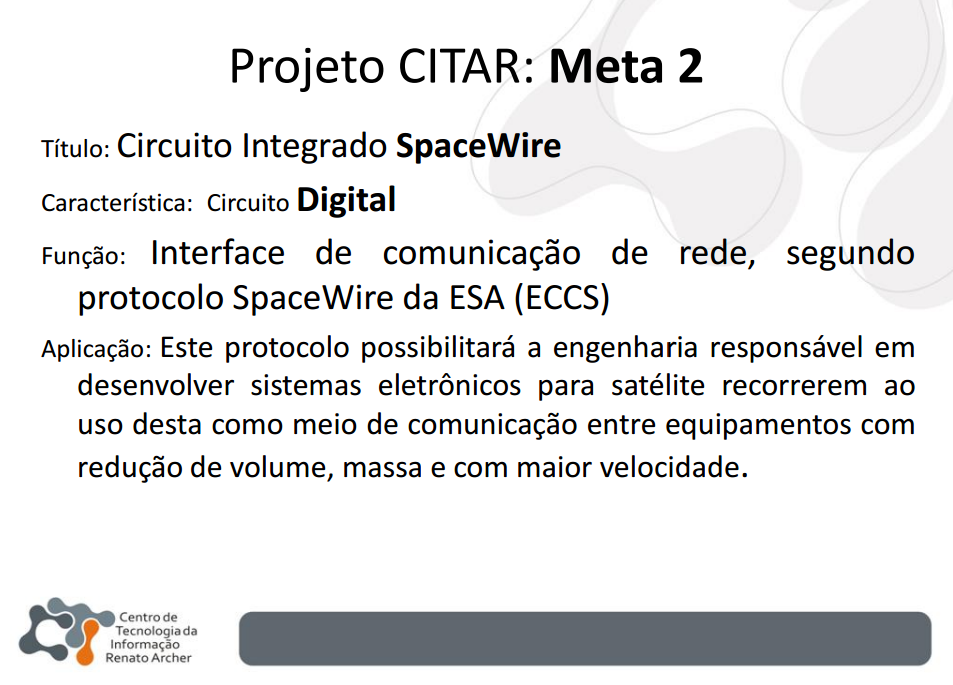
\includegraphics[scale = 0.55]{Imagens/ProjetoCitarMeta2}
	
	Fonte: site do IEAV Instituto de Estudos Avançados (2010, p. 9).\footnotemark[2]
	
	\label{Meta2}
\end{figure}

\let\thefootnote\relax\footnotetext[2]{Figura retirada da URL \url{http://www.ieav.cta.br/peice2010/Apresentacoes\_PEICE\%202010\_pdf/2010-11-29/0102-Saulo.pdf}. Acesso em: 7 out. 2015.}

\vfill

\begin{figure}[!htb]
	\centering
	\caption{Projeto CITAR - Meta 2.}
	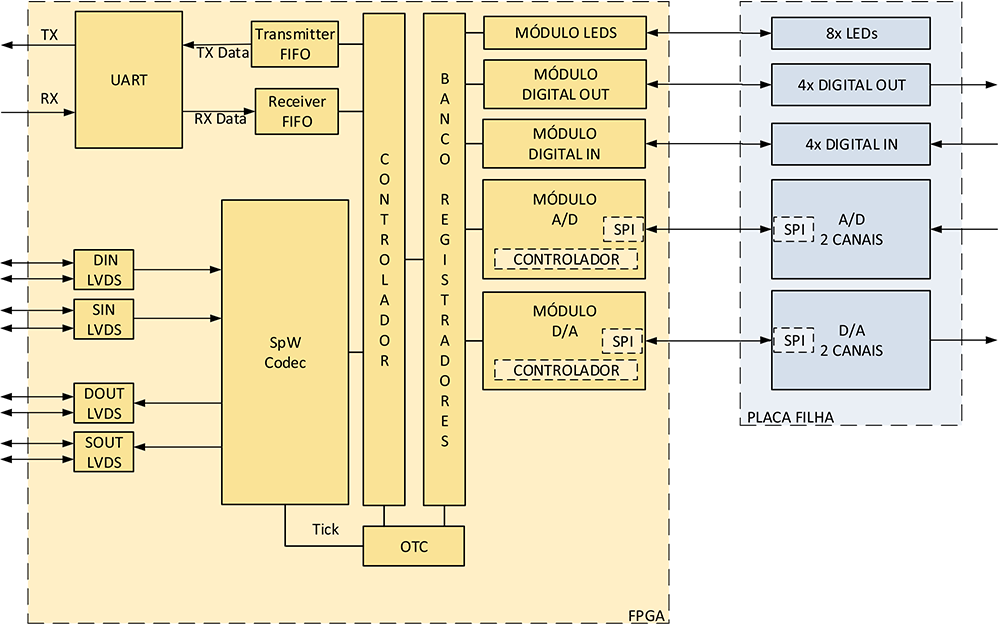
\includegraphics[scale = 1.7]{Imagens/Arch_ApSpW}
	
	Fonte: Elaborada pelo autor.
	
	\label{ArchSpW}
\end{figure}

}			% fim \afterpage
% ---

% ---
\section{Materiais e métodos}
Para o desenvolvimento do projeto foi utilizado:

\begin{itemize}
	\item Computador
	\item Software Xilinx ISE
	\item Placa de prototipagem GR-PCI-XC5V
	\item Cabo SpaceWire
\end{itemize}

Inicialmente foi realizado um estudo sobre as propriedades do protocolo SpaceWire. Em seguida, foram criados algumas aplicações utilizando o protocolo para melhor compreensão. Depois foi projetado a arquitetura proposta (Figura \ref{ArchSpW}) que possibilita o acesso aos conversores via protocolo SpW. Para todos os subsistemas um cenário de testes foi projetado, garantindo o perfeito funcionamento do sistema.

% ---


% ---
\section{Estudos, testes e simulações do codec SpaceWire}

\let\thefootnote\svthefootnote
O primeiro passo escolhido foi estudar sobre o protocolo de comunicação SpaceWire. Verificar seu funcionamento, os dados de entrada e de saída, a estrutura necessária para a sua aplicação, entre outros. O estudo se baseou inicialmente através da leitura do documento \textit{Space engineering: SpaceWire – Links, nodes, routers and networks}\footnote{Space engineering: SpaceWire – Links, nodes, routers and networks \url{http://www.ecss.nl/forums/ecss/_templates/default.htm?target=http://www.ecss.nl/forums/ecss/dispatch.cgi/standards/docProfile/100302/d20060808084754/No/t100302.htm}}, o qual descreve detalhadamente como devem ser construídos todos os níveis para sua implementação (nível das camadas física, de sinal, de caracteres, de pacotes de dados etc.). Procurou-se através deste estudo ter uma visão geral do protocolo, lembrando que o foco é a sua utilização e não a construção do mesmo.

O codec SpaceWire utilizado para estudo de teste e simulação foi desenvolvido por Jorge Luiz Nabarrete em seu trabalho de pós-doutorado no Instituto Mauá de Tecnologia em 2012.

Um dos primeiros testes com o codec foi verificar seu funcionamento ligando a saída do mesmo em sua entrada (loopback test). A simulação pôde ser visualizada através do software ISim (ISE Simulator) da Xilinx. Foram observadas várias características deste protocolo através desta simulação, entre elas, a taxa de envio de dados no início da transmissão e a alta prioridade no envio de TimeCode como está indicado na Figura \ref{SimulSpW_1}.

\begin{figure}[!htb]
	\centering
	\caption{Simulação codec SpW com interligação da saída com a entrada.}
	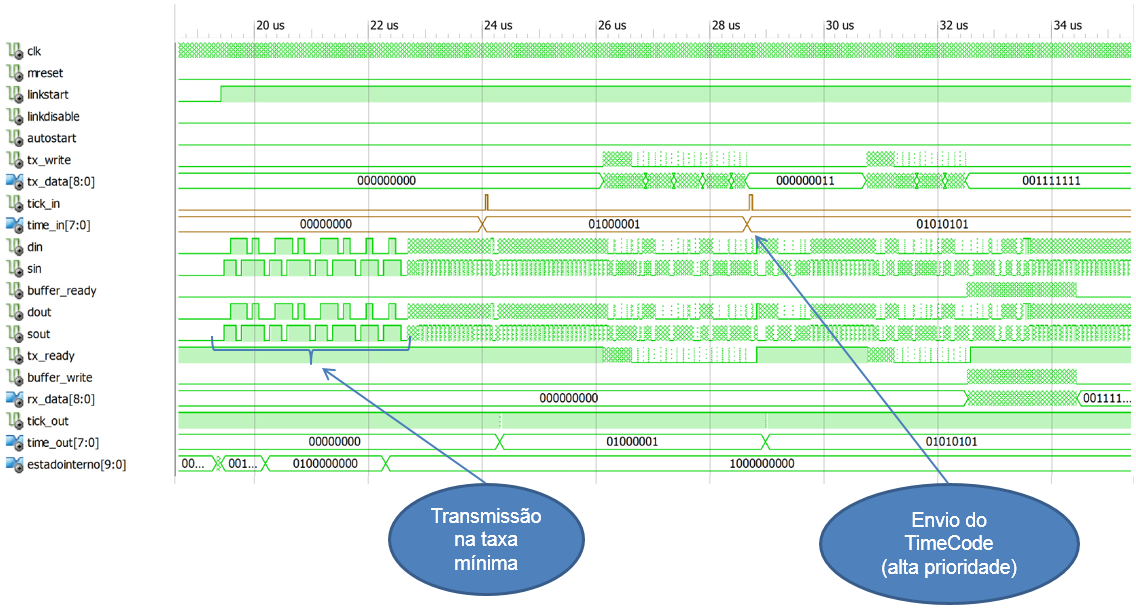
\includegraphics[scale = 0.7, angle = 90]{Imagens/SimulSpW_1}
	
	Fonte: Elaborada pelo autor.
	
	\label{SimulSpW_1}
\end{figure}

Outro teste realizado foi conectar o codec SpW que estava sendo analisado com o codec SpW que o coorientador Rafael Corsi Ferrão estava utilizando em seu projeto com a placa de desenvolvimento \textit{Altera DE4 Development and Education Board}\footnote{Altera DE4 Development and Education Board \url{http://www.terasic.com.tw/cgi-bin/page/archive.pl?Language=English\&CategoryNo=138\&No=\\501\&PartNo=1}}. Vale lembrar que os codecs SpW são de desenvolvedores diferentes. Após configurar a frequência de transmissão, vimos que os codecs se comunicavam corretamente.

Através da leitura, dos testes e simulações conseguiu-se criar uma boa base para o uso do protocolo SpaceWire e com isso dar prosseguimento no projeto.
% ---

% ---
\section{Arquitetura do sistema}

Após o estudo e análise do protocolo SpaceWire, iniciou-se o projeto da arquitetura do sistema. O objetivo desta etapa é estabelecer, de forma mais detalhada, os sinais de entrada e saída bem como os componentes a serem utilizados no sistema e suas interligações.

No inicio, a arquitetura proposta buscava mostrar de uma forma geral, o objetivo do projeto, como pode ser visualizada na figura \ref{Arch_1}.

Para a implementação do projeto, necessitou-se de uma arquitetura mais detalhada com os blocos necessários mais definidos. Após algumas modificações, chegou-se a arquitetura geral final que pode ser visualizada na figura \ref{Arch_ApSpW}. Pode-se observar a estrutura dos blocos que estão contidos na FPGA e os blocos na Placa Filha\footnote{Placa Filha: Nome dado a placa construída no projeto, a qual contém leds, saídas e entradas digitais e os conversores A/D e D/A.}.

Também foi feito uma pequena arquitetura (figura \ref{Arch_conversores}) mostrando com maior detalhe a comunicação entre os módulos A/D e D/A com seus respectivos conversores. Essa pequena arquitetura ajudou na implementação do código VHDL dos módulos, pois permitiu visualizar as entradas e saídas necessárias da comunicação SPI (Serial Peripheral Interface) com os conversores.

Os conversores utilizados no projeto são: o analógico-digital MCP3204\footnote{\label{MCP3204}Datasheet do conversor A/D MCP3204: \url{http://ww1.microchip.com/downloads/en/DeviceDoc/21298c.pdf}. Acesso em: 12 out. 2015.} e o digital-analógico MCP4922\footnote{\label{MCP4922}Datasheet do conversor D/A MCP4922: \url{http://ww1.microchip.com/downloads/en/DeviceDoc/22250A.pdf}. Acesso em: 12 out. 2015.}, ambos da Microchip. Foram escolhidos estes conversores pois oferecem interface de comunicação SPI, possuem no mínimo dois canais de leitura/escrita e uma boa resolução (12 bits). Procurou-se com estes conversores criar uma aplicação que pudesse ser bem genérica, podendo conectá-los a quatro equipamentos como motores e sensores.

\begin{figure}[!htb]
	\centering
	\caption{Primeira arquitetura do projeto Aplicação SpaceWire.}
	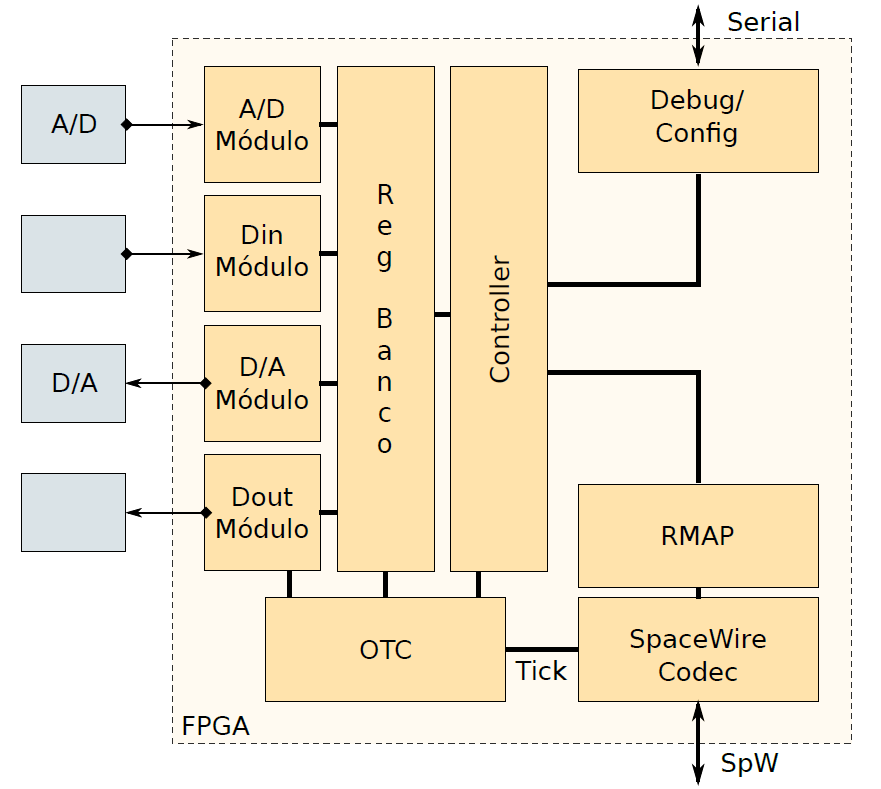
\includegraphics[scale = 0.5]{Imagens/Arch_1.png}
	
	Fonte: Elaborada pelo autor.
	
	\label{Arch_1}
\end{figure}

\begin{figure}[!htb]
	\centering
	\caption{Arquitetura geral do projeto Aplicação SpaceWire.}
	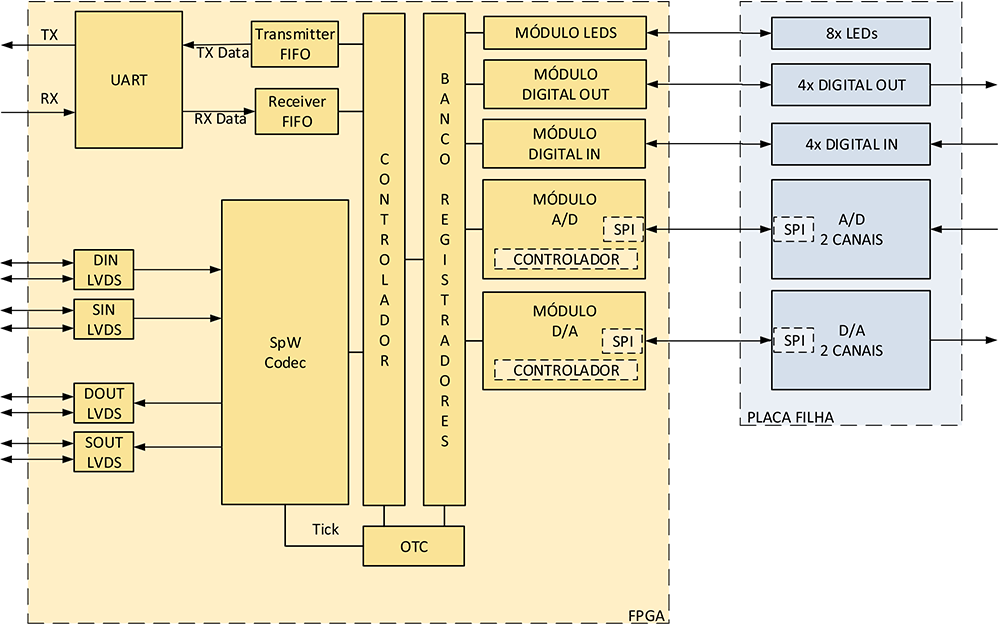
\includegraphics[scale = 1.85]{Imagens/Arch_ApSpW}
	
	Fonte: Elaborada pelo autor.
	
	\label{Arch_ApSpW}
\end{figure}

\begin{figure}[!htb]
	\centering
	\caption{Arquitetura entre os módulos A/D e D/A e seus respectivos conversores.}
	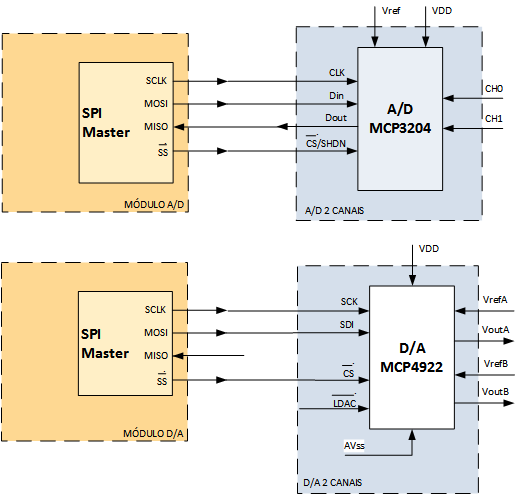
\includegraphics[scale = 0.9]{Imagens/Arch_conversores}
	
	Fonte: Elaborada pelo autor.
	
	\label{Arch_conversores}
\end{figure}

% ---

\vfill

% ---
\section{Construção do hardware (Placa Filha)}

Foi construído um hardware, chamado Placa Filha (figura \ref{PlacaFilha}), contendo: oito leds, seis entradas/saídas digitais, um coversor A/D MCP3204 e um convesor D/A MCP4922. Esta placa foi projetada com o intuito de ser conectada a placa de desenvolvimento GR-PCI-XC5V através de uma placa expansora de pinos GR-CPCI-TEST da Aeroflex Gaisler (figura \ref{cpci-test} e figura \ref{PlacaFilha_GRPCI}).

A placa foi projetada utilizando o programa EAGLE PCB Design Software\footnote{Informações sobre o CadSoft EAGLE: \url{http://www.cadsoftusa.com/eagle-pcb-design-software/about-eagle/}. Acesso em 12 out. 2015.} e confeccionada em uma máquina LPKF disponibilizada pelo Instituto Mauá de Tecnologia.

Esta placa permite que testes práticos possam ser realizados e mostrar o real funcionamento do sistema.

\begin{figure}[!htb]
	\centering
	\caption{Foto da Placa Filha conectada na placa expansora GR-CPCI-TEST.}
	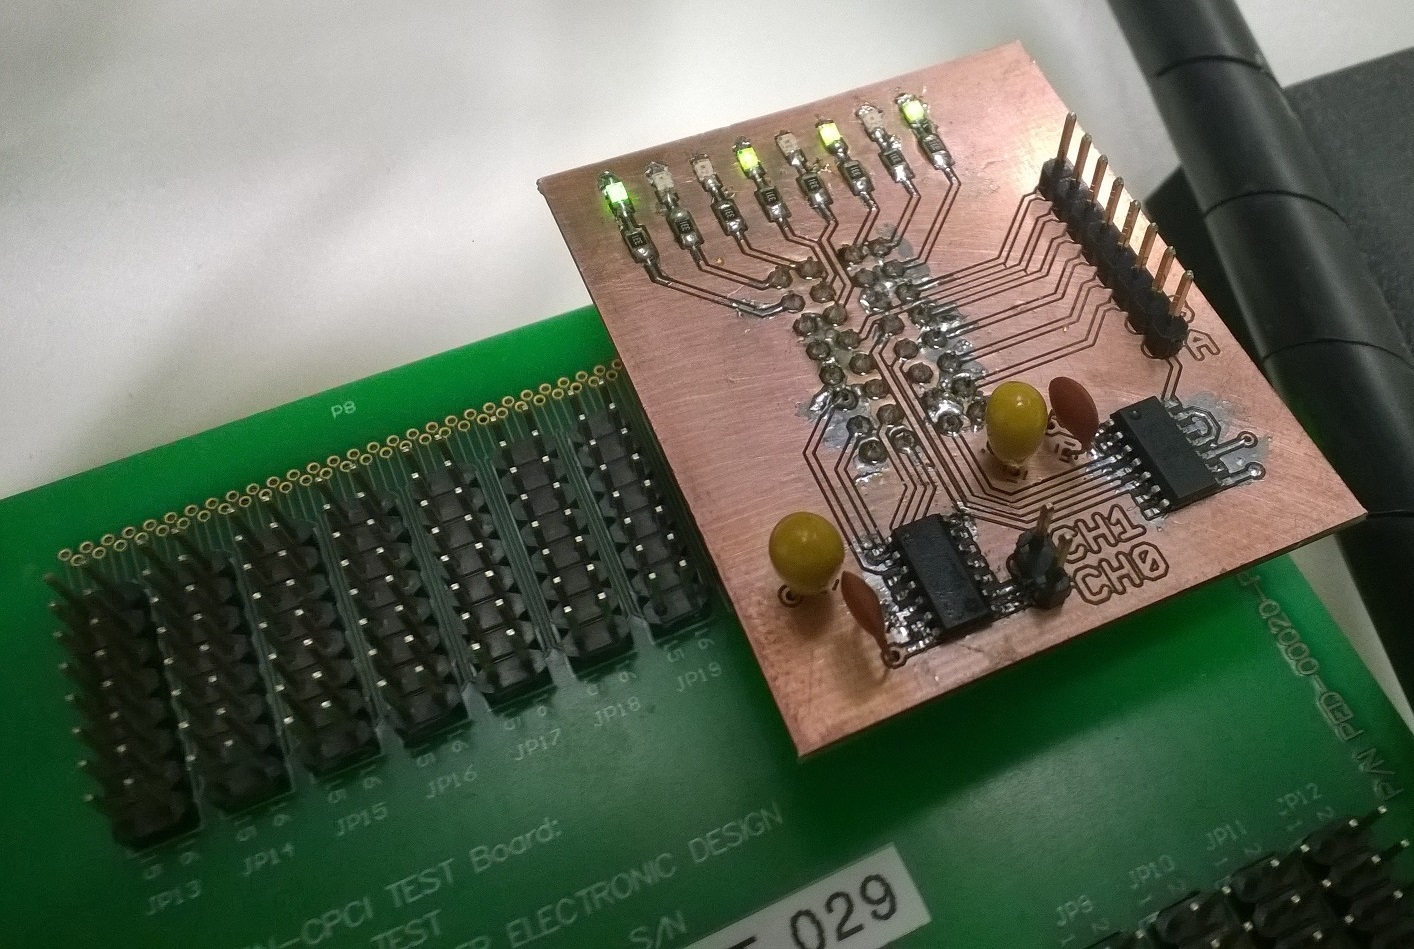
\includegraphics[scale = .4]{Imagens/PlacaFilha}
	
	Fonte: Elaborada pelo autor.
	
	\label{PlacaFilha}
\end{figure}

\begin{figure}[!htb]
	\centering
	\caption{GR-CPCI-TEST}
	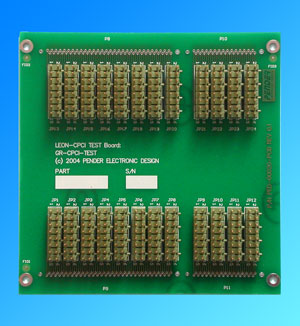
\includegraphics[scale = .9]{Imagens/cpci-test}
	
	Fonte: GAISLER.
	
	\label{cpci-test}
\end{figure}

\begin{figure}[H]
	\centering
	\caption{Placa Filha, GR-PCI-TEST e GR-PCI-XC5V.}
	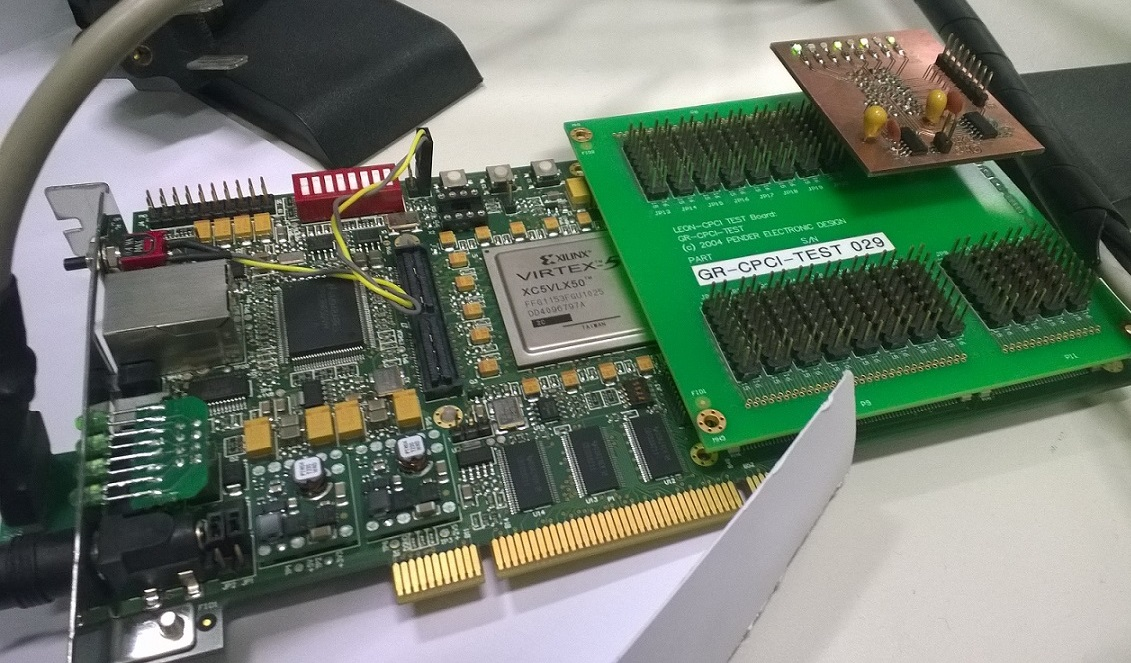
\includegraphics[scale = .8, angle = 90]{Imagens/PlacaFilha_GRPCI}
	
	Fonte: Elaborada pelo autor.
	
	\label{PlacaFilha_GRPCI}
\end{figure}

% ---

\section{Implementação, simulação e teste do módulo digital-analógico com o conversor D/A MCP4922}

Através da Placa Filha pôde-se finalmente realizar testes com os conversores. Mas antes disso, é necessário fazer a implementação dos módulos e realizar simulações em software antes de efetivamente executá-los na prática. É muito importante o uso da simulação em software, pois se o subsistema não funcionar na simulação, muito provavelmente não funcionará na prática.

Para a implementação do módulo digital-analógico através da programação em VHDL, construi-se, primeiramente, um diagrama de blocos do controlador do módulo para melhor compreensão e organização da estrutura do código. Este diagrama é mostrado na figura \ref{controlador_DAC}. Foi utilizado como referência para a contrução do diagrama a máquina de Moore onde as saídas são determinadas pelo estado corrente apenas (e não pela entrada). 

O controlador do módulo D/A controla os sinais do módulo SPI que é por onde os dados são enviados e recebidos do conversor. Inicialmente o controlador espera chegar um dado novo no registrador para começar o processo de envio do dado ao canal do conversor requisitado. Após iniciado o processo de envio do dado, o mesmo entra em um novo estado de espera até que o último bit seja enviado. Logo depois, o controlador verifica se há um dado a ser enviado ao outro canal do conversor, evitando com que um canal tenha maior prioridade.

Foi realizado um teste na prática para ver este sistema funcionando. Neste teste estava sendo utilizado: o banco de registradores, o módulo A/D e o conversor A/D MCP4922. O registrador ficava recebendo dados em um endereço específico e enquanto isso o controlador do módulo verificava se havia um dado novo a ser enviado ao D/A. Toda vez que um dado era escrito no registrador, o controlador enviava este dado via SPI para o conversor MCP4922. O sinal analógico do conversor pôde ser observado através de um osciloscópio. A foto do teste realizado pode ser visualizada na figura \ref{teste_conversor_DAC}.

\begin{figure}[!htb]
	\centering
	\caption{Diagrama de blocos do controlador do módulo digital-analógico.}
	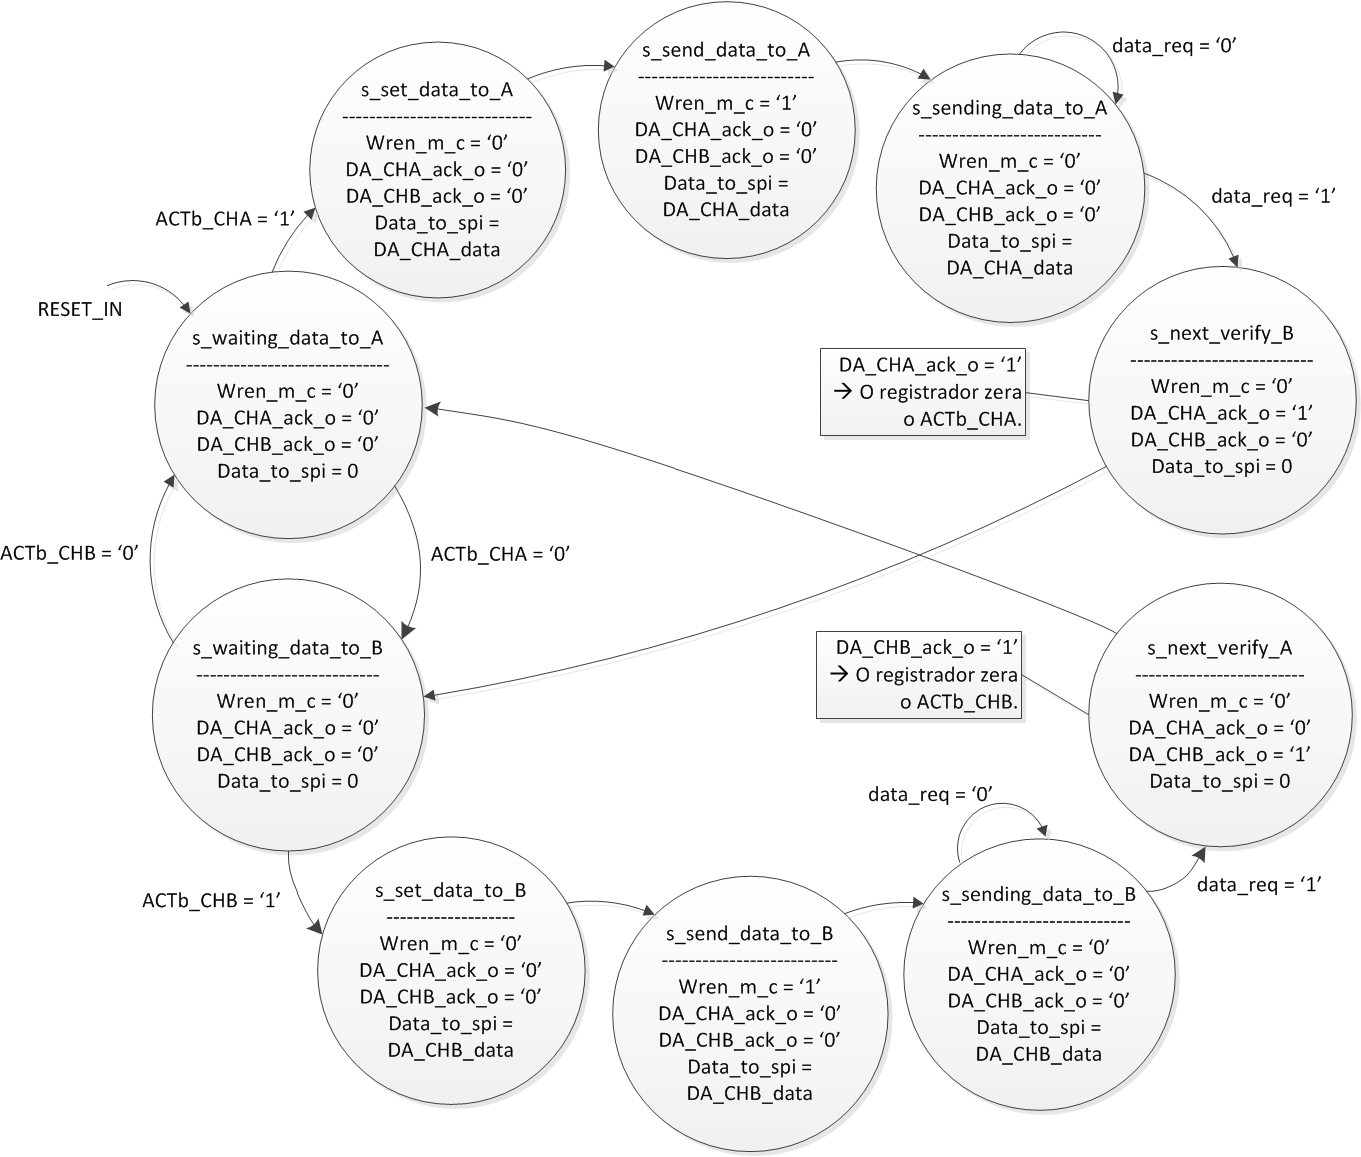
\includegraphics[scale = .9]{Imagens/controlador_DAC}
	
	Fonte: Elaborada pelo autor.
	
	\label{controlador_DAC}
\end{figure}

\begin{figure}[!htb]
	\centering
	\caption{Diagrama de blocos do controlador do módulo digital-analógico.}
	\includegraphics[scale = .7, angle = 90]{Imagens/teste_conversor_DAC}
	
	Fonte: Elaborada pelo autor.
	
	\label{teste_conversor_DAC}
\end{figure}

% ---